\chapter{Etapas de Salida de Amplificadores. }\label{salida}

\hspace{10pt} La etapa de salida en un amplificador es la encargada de suministrar los niveles  de señal y de potencia requeridos a una carga determinada. Las principales características de las etapas de salida en amplificadores son:

\begin{itemize}
	\item Presentar baja resistencia de salida, para que la señal entregada a la carga tienda a ser independiente de ésta.  
	\item En general deben poder manejar niveles de señales relativamente grandes, por lo que se deben utilizar en los dispositivos involucrados modelos de gran señal.
	\item La linealidad suele ser un requisito muy importante, por lo que se debe diseñar para reducida distorsión armónica.
	\item Se debe entregar la potencia requerida a la carga de un modo eficiente , es decir que la potencia disipada en los dispositivos activos de la etapa de salida debe ser lo más baja posible con respecto a la potencia entregada a la carga.
\end{itemize}

 Los amplificadores se clasifican de acuerdo con la forma de onda de corriente del o de los dispositivos activos que controlan la salida.

Las etapas de salida en clase A, ver figura \ref{clases1} a), el dispositivo activo de salida conduce todo el ciclo de una onda senoidal tomada como referencia. Producen en general una gran disipación de potencia en los dispositivos utilizados y por lo tanto presentan un bajo rendimiento.

Las etapas de salida en clase B,  mostrada en la figura \ref{clases1}) b), mejoran este problema al tener una casi nula disipación de potencia si la señal de entrada es cero. Para entregar la potencia a la salida se utilizan al menos dos dispositivos activos conduciendo medio ciclo cada uno en forma alternada. El rendimiento de las etapas de salida clase B es mayor que las de clase A, siendo idealmente el máximo rendimiento alcanzado del 78.54\%. Las principales aplicaciones de estas etapas de salida son en: etapas de salida de amplificadores de audio discretos e integrados y en etapas de salida de circuitos integrados en general.

Una variante del tipo anterior es la etapa de salida clase AB que se muestra en la figura \ref{clases1} c). En este caso los dispositivos activos de salida conducen un poco más de la mitad del ciclo cada uno, solapándose un pequeña porción del ciclo. Esto redunda en una mejora en las características de distorsión sin afectar apreciablemente al rendimiento, como se mostrará en los puntos siguientes.


Los amplificadores clase C, son aquellos en que el dispositivo activo que controla la salida conduce menos de la mitad del tiempo y es mostrado en la figura \ref{clases1} d), con esta configuración se pueden obtener rendimientos cercanos al 100\%.

\begin{figure}
	\centering
	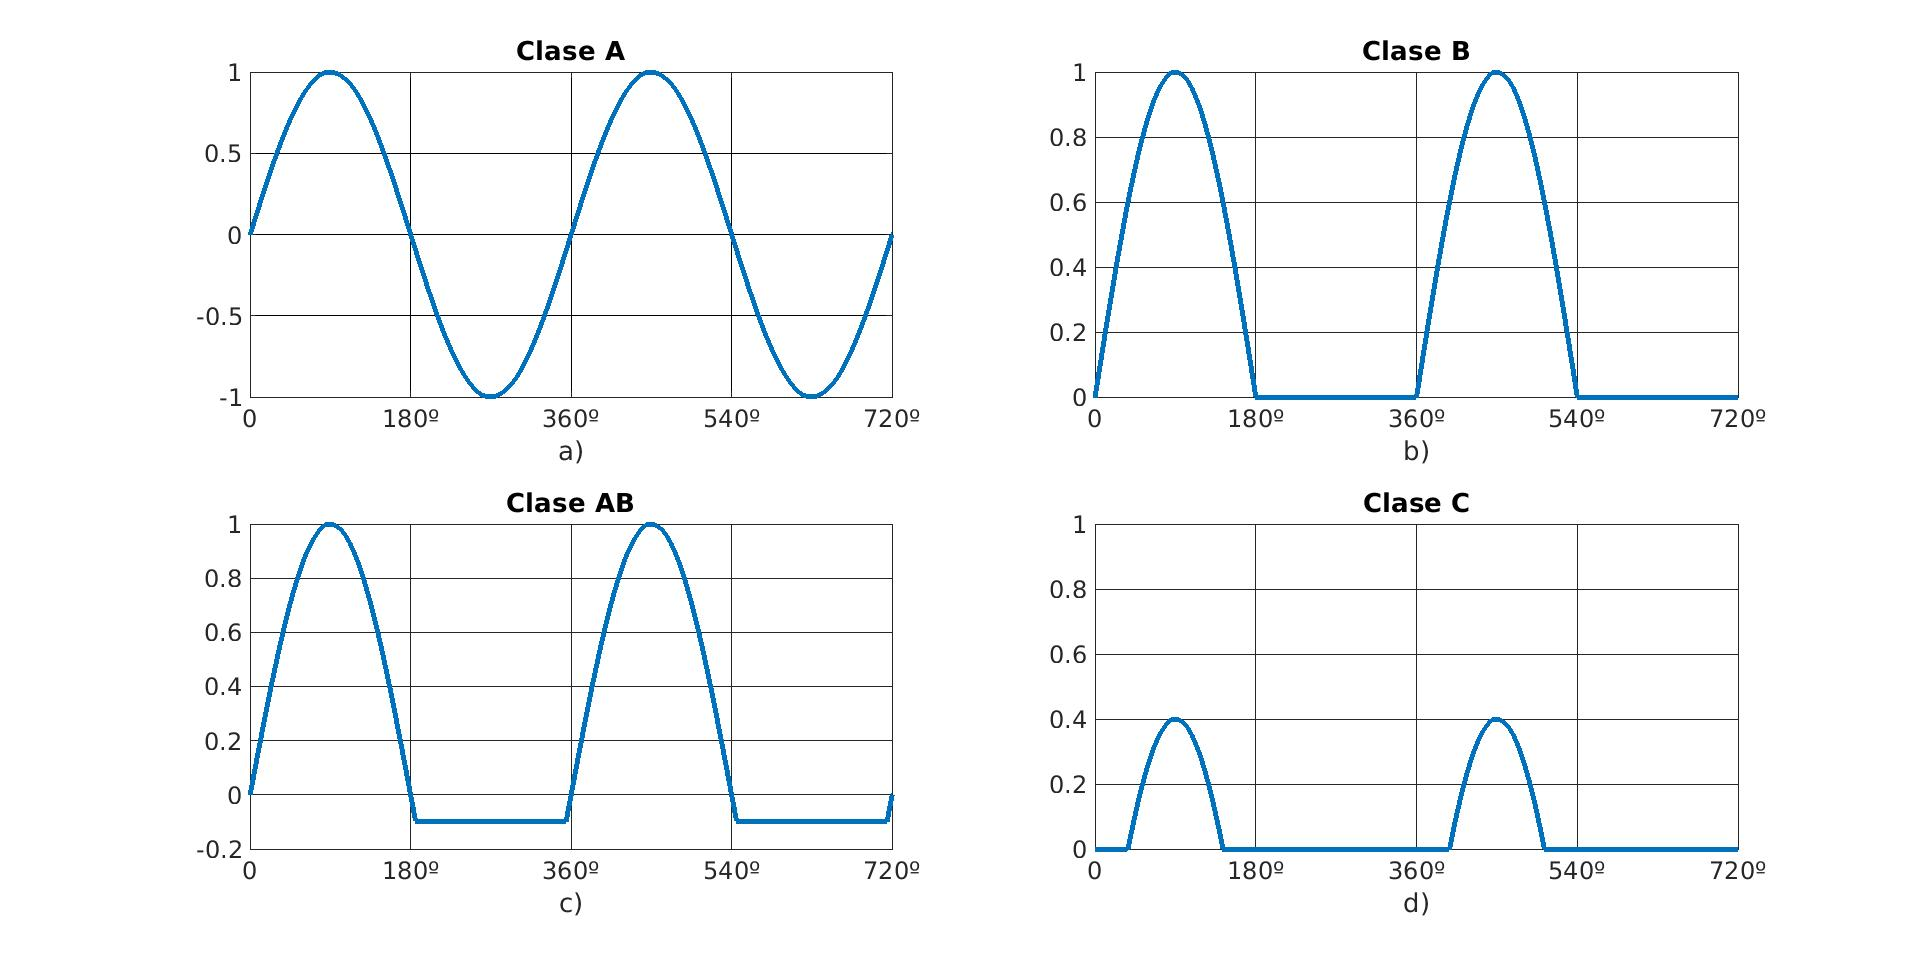
\includegraphics[width=1.0\linewidth]{figuras/claseabyc.jpg}
	\caption{Amplificadores: a)Clase A, b) Clase B, c) Clase AB y d) Clase C.}
	\label{clases1}
\end{figure}

\section{Etapa de salida Clase A}

\hspace{10pt} En la figura \ref{clases2} se muestra una etapa de salida Clase A implementada en una configuración seguidor de emisor utilizando Transistores Bipolares. El transistor $Q_1$ actúa com seguidor de emisor y el $Q_2$ como fuente de corriente continua para polarizar a $Q_1$. A la derecha de la figura se despliega el resultado del punto de operación, en especial se ve que el punto de polarización es: $I_{c1}= 37,49mA$, $I_{c2}= 39,97mA$  y $V_{s}=-0,758V$. Por lo que está polarizado de modo que  aproximadamente pueda excursionar entre $+/-$ las fuentes de alimentación ($12V$).



Esta configuración de salida posee buena linealidad y baja impedancia de salida por tratarse de un seguidor de emisor, el principal inconveniente que presenta es que la eficiencia con respecto a la entrega de potencia es baja por lo que no es utilizada cuando la potencia a entregar a una carga es elevada. Dicha eficiencia se suele cuantificar con el rendimiento:


\begin{equation}\label{ecuclases1}
	\eta=\frac{P_L}{P_T}100\%
\end{equation}

Siendo $P_L$ la potencia útil de señal entregada a una carga y $P_T$ la potencia total entregada por las fuentes de alimentación. Se puede demostrar (ver \cite{sedra99}) que en el mejor de los casos se podría obtener un $\eta=25\%$, disipándose mucha potencia en los dispositivos activos. 

\begin{figure}
	\centering
	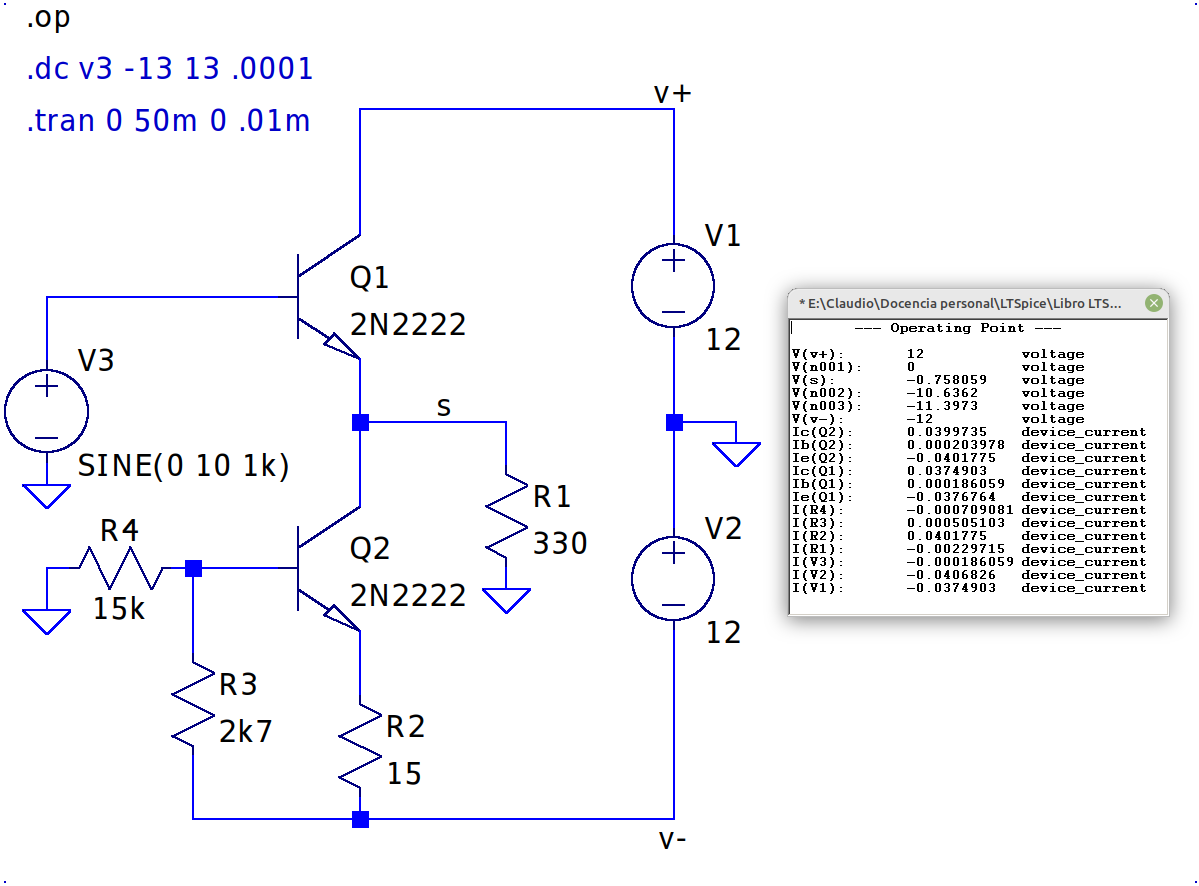
\includegraphics[width=1.0\linewidth]{figuras/claseabyc2.png}
	\caption{Seguidor de Emisor como etapa de salida Clase A.}
	\label{clases2}
\end{figure}


En la figura \ref{clases3} se muestra la salida $V_s$ en función de la entrada $V_3$ utilizando \textit{.dc v3 -13 13 .0001}, se ve en ella que dicha transferencia es aproximadamente lineal, que la saturación de $Q_1$ limita la excursión positiva y que la saturación de $Q_2$ más la caída en $R_2$ limita la negativa. 

Utilizando la directiva \textit{.tran 0 50m 0 .01m} se obtiene la respuesta temporal del circuito de la figura \ref{clases2} a la fuente de entrada senoidal $V_3$ de $10V$ de amplitud y $1KHz$ de frecuencia. En la figura \ref{clases4} se muestra en la parte inferior la salida $V_s$, del gráfico se obtiene que el valor pico a pico de la salida es de $\approx 19,87V$, por lo que la potencia media de señal entregada a la carga $R_1$  es:

\begin{equation}\label{ecuclases2}
	P_L=\frac{\displaystyle \hat{V_s}^2}{\displaystyle 2R_1}=\frac{(\displaystyle  \frac{19,87V}{2})^2}{2\times 330\Omega}=149.55mW
\end{equation}

En la parte superior de la figura mencionada se grafica la potencia instantánea entregada a la carga,  $V_s\times I(R_1)$. Si se coloca el cursor del mouse sobre la definición de la señal $V_s\times I(R_1)$ y se presionan simultáneamente el botón izquierdo del mismo y la tecla Ctrl se despliega la ventana de datos mostrada. En ella se ve que la potencia media es $151,43mW$, levemente mayor a la calculada anteriormente debido a que en este caso se computa la pequeña potencia de continua presente debido a que la tensión $V_s$ de polarización es de $-0,758V$ (ver figura \ref{clases2}). De la figura \ref{clases2} se obtienen las corrientes de polarización de los transistores que son: $I_C(Q_1)=37,4403mA$ e $I_E(Q_2)=40,1775mA$, de estos valores se obtiene que la potencia total entregada por las fuentes de alimentación es: $P_T = V_1I_C(Q_1)+V_2 I_E(Q_2)=12V\times 37,4403mA+12V\times 40,1775mA= 932,0136mW$. Por lo tanto el rendimiento de este circuito bajo estas condiciones de funcionamiento será:

 \begin{equation}\label{ecuclases3}
 	\eta=\displaystyle \frac{P_L}{P_T}\times 100=\frac{149,55mW}{932,0136mW}\times 100\approx16.05\%
 \end{equation}

De un modo similar a como se obtuvo la potencia media en la carga, se puede calcular la potencia disipada en cada componente del circuito, por ejemplo para dimensionar la potencia media disipada en $Q_1$, se grafica la potencia instantánea de la señal $V_{ce1}\times I_c(Q_1)$ y se despliega la ventana de datos como se explicó anteriormente obteniendo el valor medio buscado, en las condiciones de funcionamiento del circuito del ejemplo dio: $P_D(Q_1)=320,28mW$. 

\begin{figure}
	\centering
	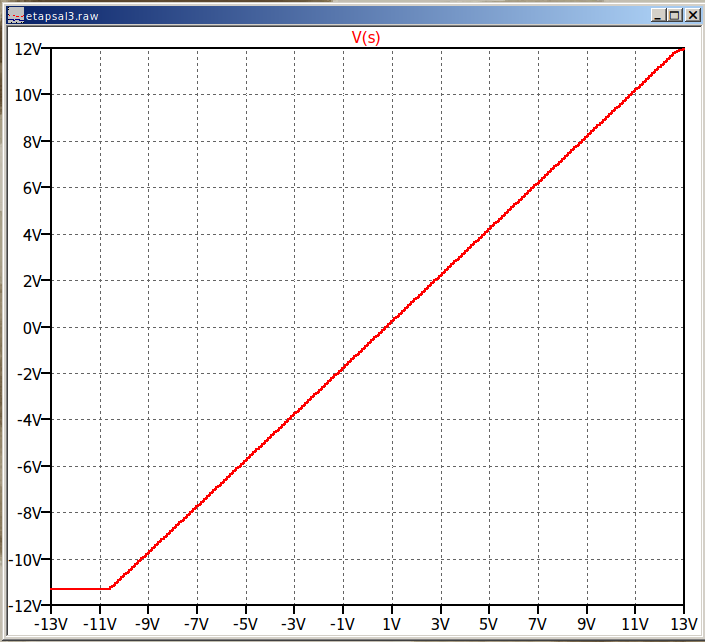
\includegraphics[width=0.7\linewidth]{figuras/claseabyc3.png}
	\caption{Transferencia del circuito de la figura \ref{clases2}.}
	\label{clases3}
\end{figure}

\begin{figure}
\centering
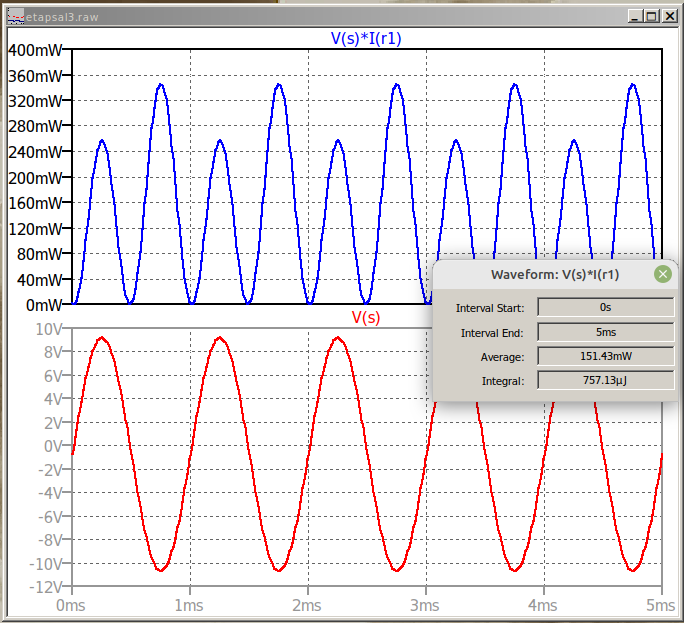
\includegraphics[width=0.8\linewidth]{figuras/claseabyc4.png}
\caption{Salida $V_s$ y potencia sobre $R_1$.}
\label{clases4}
\end{figure}


\section{Etapas de salida Clase B y AB}

\hspace{10pt} Las etapas de salida en clase A producen una gran disipación de potencia en los dispositivos de salida en proporción a la potencia útil entregada ( bajo rendimiento), inclusive en el caso en que no exista entrada de corriente alterna. En muchas aplicaciones de amplificadores de potencia, el circuito puede estar largos períodos de tiempo en estado de espera sin señal de entrada, o con entrada intermitente, como en el caso de
señales de voz. La potencia disipada en estos períodos es desperdiciada, esto implica desperdicio de potencia entregada por la fuente de alimentación, y aumento de la disipación en los dispositivos activos y por lo tanto aumento de la temperatura de operación de los mismos. La potencia disipada en los dispositivos activos afecta el tamaño físico
requerido por ellos y sus disipadores, y por lo tanto se deben utilizar dispositivos más costosos (dispositivos discretos de mayor tamaño y más requerimiento de área de silicio en dispositivos integrados).
Las etapas de salida en clase B  y AB mejoran este problema, al tener una casi nula disipación de potencia si la señal de entrada es cero. Para entregar la potencia a la salida se utilizan  al menos dos dispositivos
activos conduciendo medio ciclo cada uno en forma alternada. El rendimiento de las etapas de salida clase B es mayor que las de clase A, siendo idealmente el máximo rendimiento alcanzado del $78,5 \%$. Las principales aplicaciones de estas etapas de salida son en: Etapas de salida de amplificadores de audio discretos e integrados y en etapas de salida de circuitos integrados en general.

En la figura \ref{clases5} se muestra la configuración básica manejada por tensión de una etapa de salida en clase B. En ella se ve que los dispositivos de salida  $Q_1$ y $Q_2$ son transistores bipolares complementarios, siendo éstos idealmente iguales. En el ciclo positivo de la tensión de entrada $V_i$ el transistor $Q_1$ conduce y el transistor $Q_2$ se mantiene cortado, produciéndose el ciclo positivo de la tensión de salida $V_o$. Ocurre lo inverso en el ciclo negativo de la tensión de entrada ( $Q_1$ está cortado y $Q_2$ conduciendo). La figura \ref{clases6} muestra la simulación temporal de la respuesta del circuito a una entrada $V_i$ senoidal de amplitud $5V$ y frecuencia $1KHz$, en dicha figura se ve en los dos gráficos inferiores las corrientes de colector de los transistores $Q_1$ y $Q_2$ mostrando la conducción alternada ya mencionada. Los gráficos superiores muestran: la corriente en la carga y la tensión en la salida, en ella se ve el efecto de las tensiones de umbral de ambos transistores que producen la denominada distorsión por cruce, típico de las etapas de salida clase B.

En la figura \ref{clases7} se traza la curva de transferencia utilizando el barrido de continua de la fuente $V_i$, en dicha curva se ve que las pendientes en las zonas de conducción de los dispositivos activos son aproximadamente igual a uno (esto se debe a que actúan como seguidores de emisor). También se nota la distorsión por cruce debido a que los transistores están polarizados al corte, necesitando vencer el umbral de conducción de su tensión Base-Emisor y la saturación de los transistores  para tensiones de entrada cercanas a las fuentes de alimentación. Es de notar que la máxima excursión simétrica está delimitada por esta última condición.


\begin{figure}
	\centering
	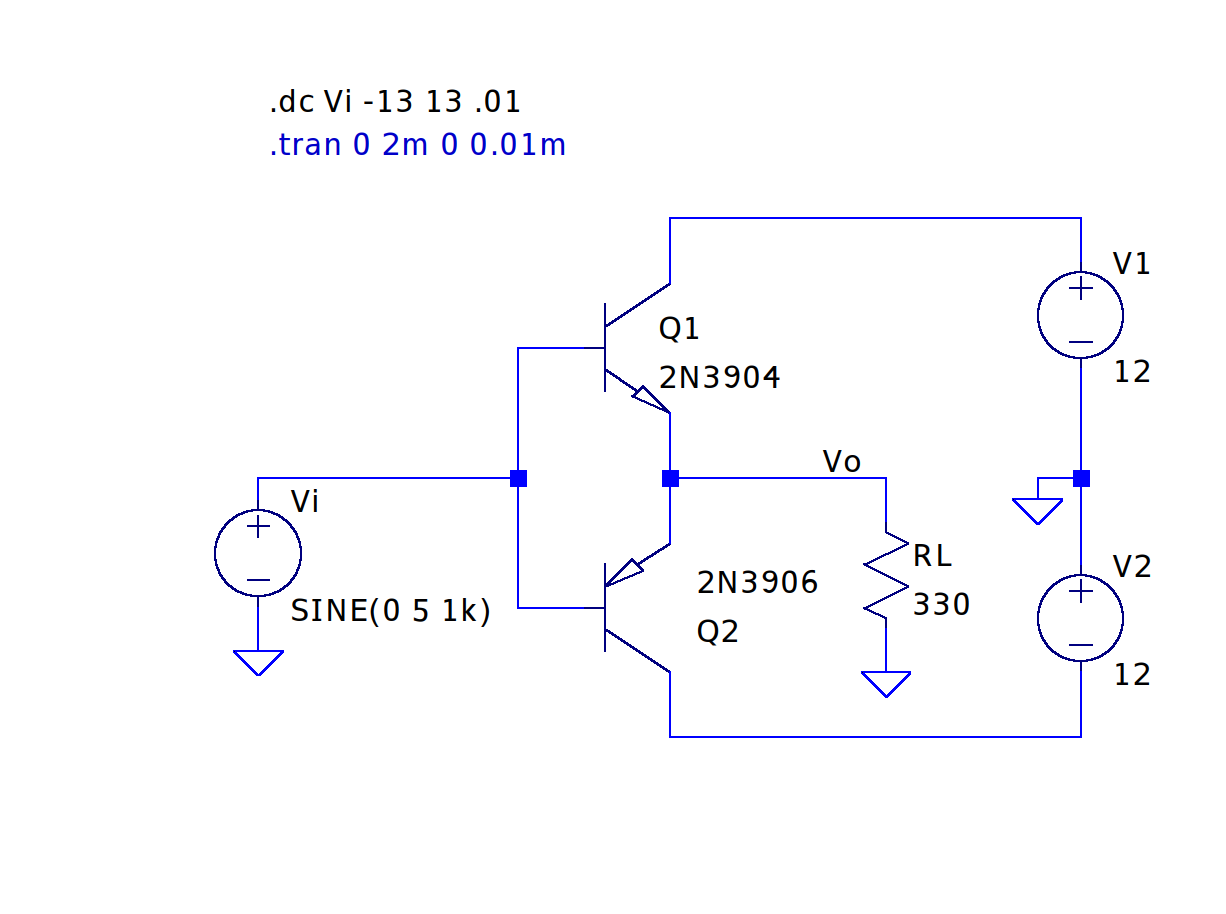
\includegraphics[width=0.8\linewidth]{figuras/claseabyc5.png}
	\caption{Etapa de salida clase B controlada por tensión.}
	\label{clases5}
\end{figure}

\begin{figure}
	\centering
	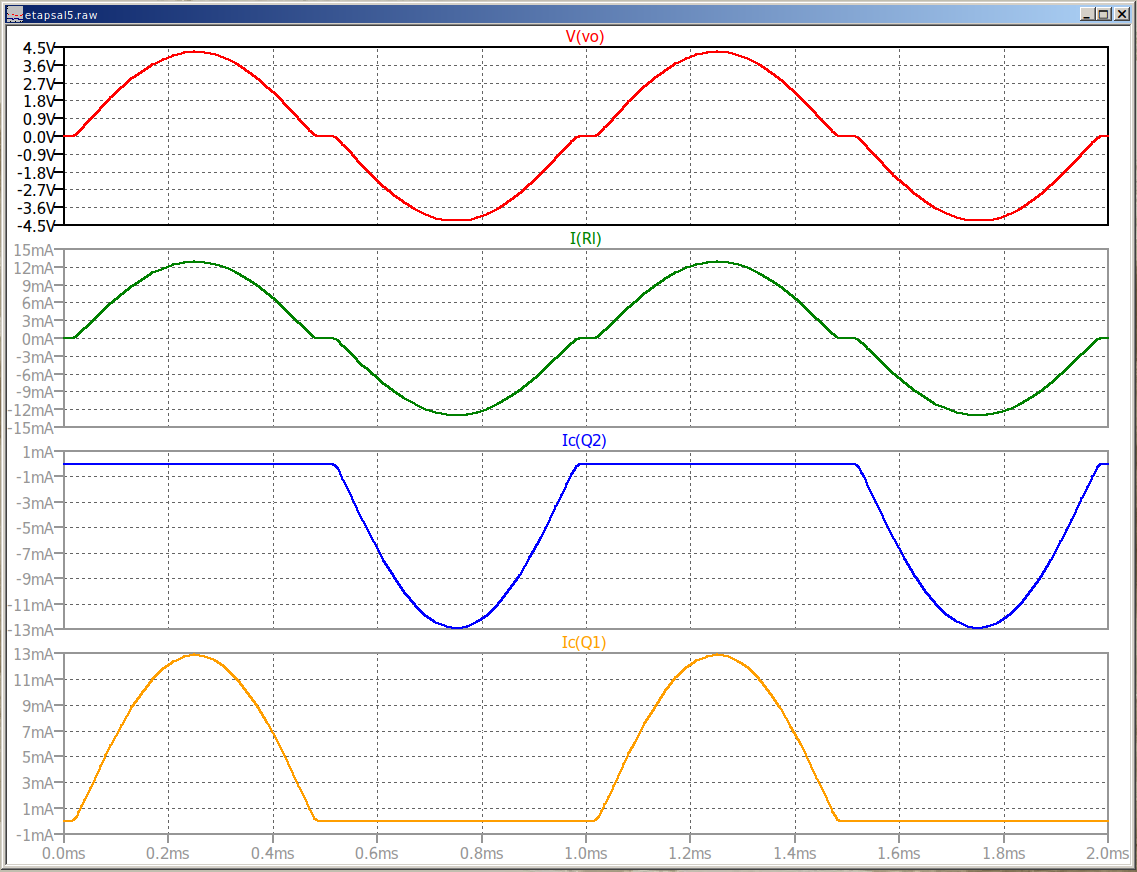
\includegraphics[width=0.8\linewidth]{figuras/claseabyc6.png}
	\caption{Respuesta temporal de una etapa clase B controlada por tensión}
	\label{clases6}
\end{figure}

\begin{figure}
	\centering
	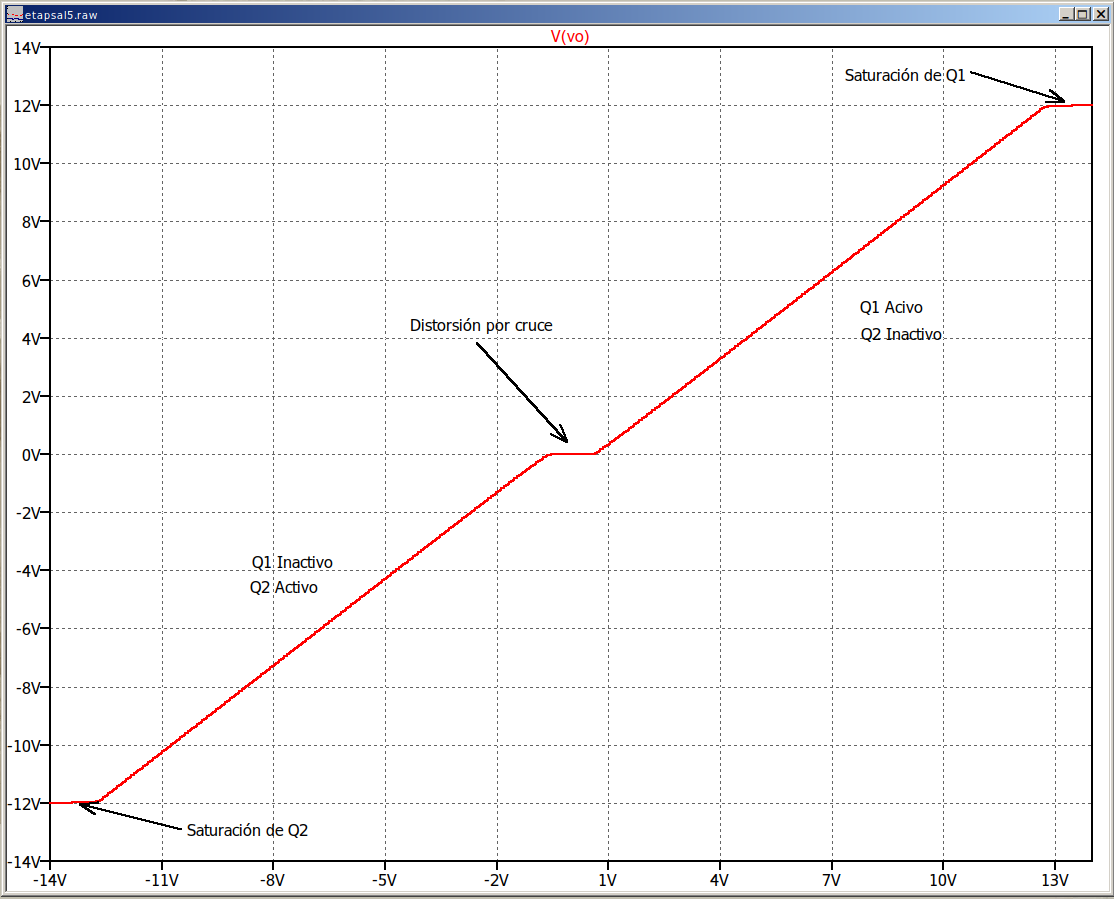
\includegraphics[width=0.8\linewidth]{figuras/claseabyc7.png}
	\caption{Transferencia de una etapa clase B controlada por tensión.}
	\label{clases7}
\end{figure}


Otra posible configuración es la mostrada en la figura \ref{clases8} En 
 este caso, la etapa de salida es manejada por el transistor $Q_3$, este transistor trabaja en clase A y está polarizado de modo que su corriente de polarización $I_C(Q_3)$ sea aproximadamente igual a $I_Q$, corriente que entrega el generador de continua ubicado en la parte superior del esquema. De tal modo los transistores $Q_1$ y $Q_2$ están polarizados al corte, y dado que son complementarios e idealmente iguales, la tensión de salida sin señal de alterna es de $0V$. 
 
 \begin{figure}
 	\centering
 	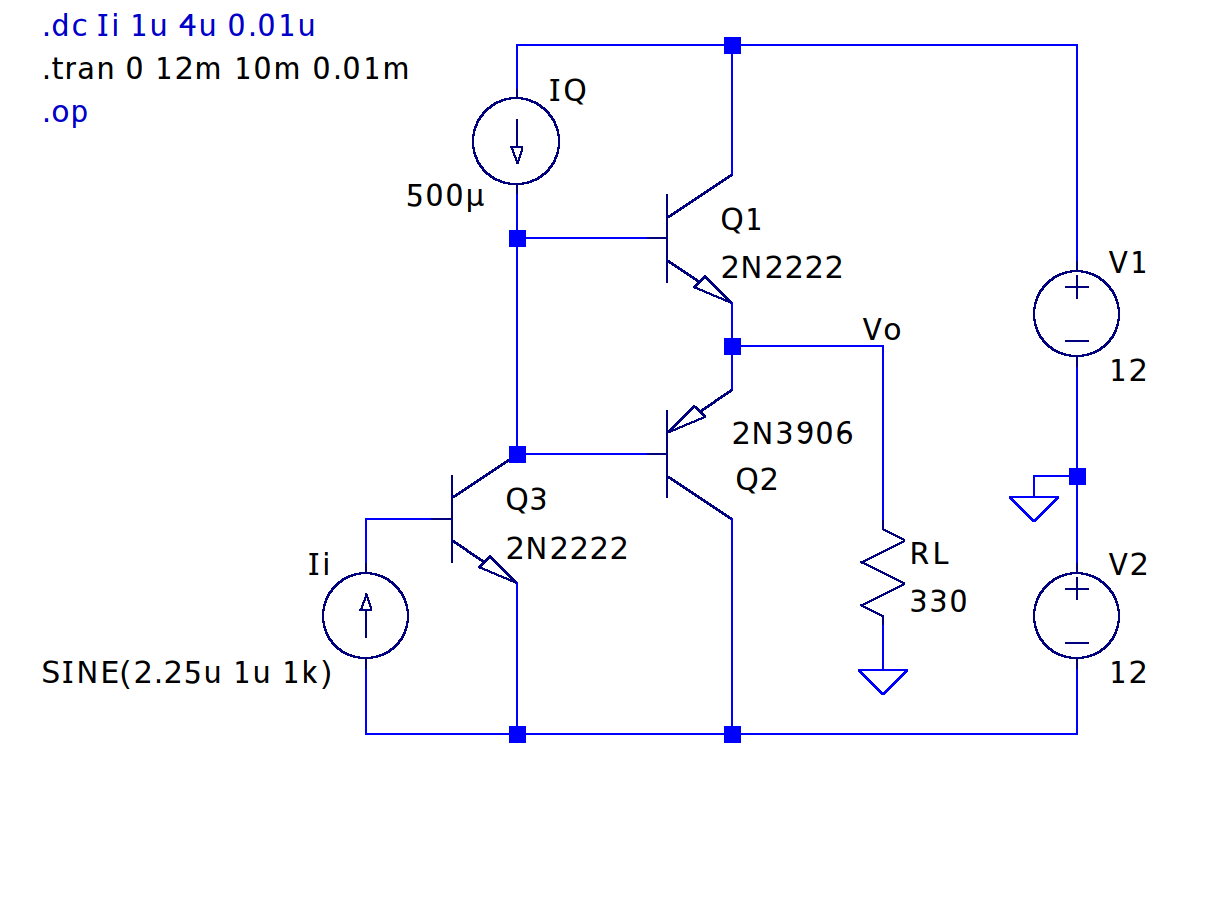
\includegraphics[width=0.8\linewidth]{figuras/claseabyc8.png}
 	\caption{Respuesta temporal de una etapa clase B controlada por corriente.}
 	\label{clases8}
 \end{figure}
 
 Idealmente esta configuración permitiría, como en el caso anterior, una máxima excursión de salida limitada sólo por la saturación de los transistores de salida, aunque para lograr esto debe asegurarse que el transistor $Q_3$ no entre en corte antes de que se produzca la saturación del transistor $Q_1$ en el semiciclo positivo de la tensión de salida. Es decir debe asegurarse que:


 \begin{equation}\label{ecuclases4}
	I_Q>\displaystyle \frac{V_1-V_{ce_1sat}}{(\beta + 1)R_L}
\end{equation}

En el caso en que $I_Q$ sea menor que el valor anterior, la máxima excursión positiva de la tensión de salida estará limitada por el corte de $Q_3$ y será $I_Q (\beta + 1)R_L$.

En la figura \ref{clases9} se traza la curva de transferencia utilizando el barrido de continua de la fuente de corriente de base de $Q_3$ $I_i$, en dicha curva se ve que las pendientes en las zonas de conducción de los dispositivos activos no son tan lineales como en el caso anterior debido a que $Q_3$ está en Clase A trabajando a gran señal (estas no linealidades se compensan en un diseño completo con realimentación global). También se nota, como en el caso anterior, la distorsión por cruce y la saturación de los transistores  para tensiones de salida cercanas a las fuentes de alimentación.

 \begin{figure}
	\centering
	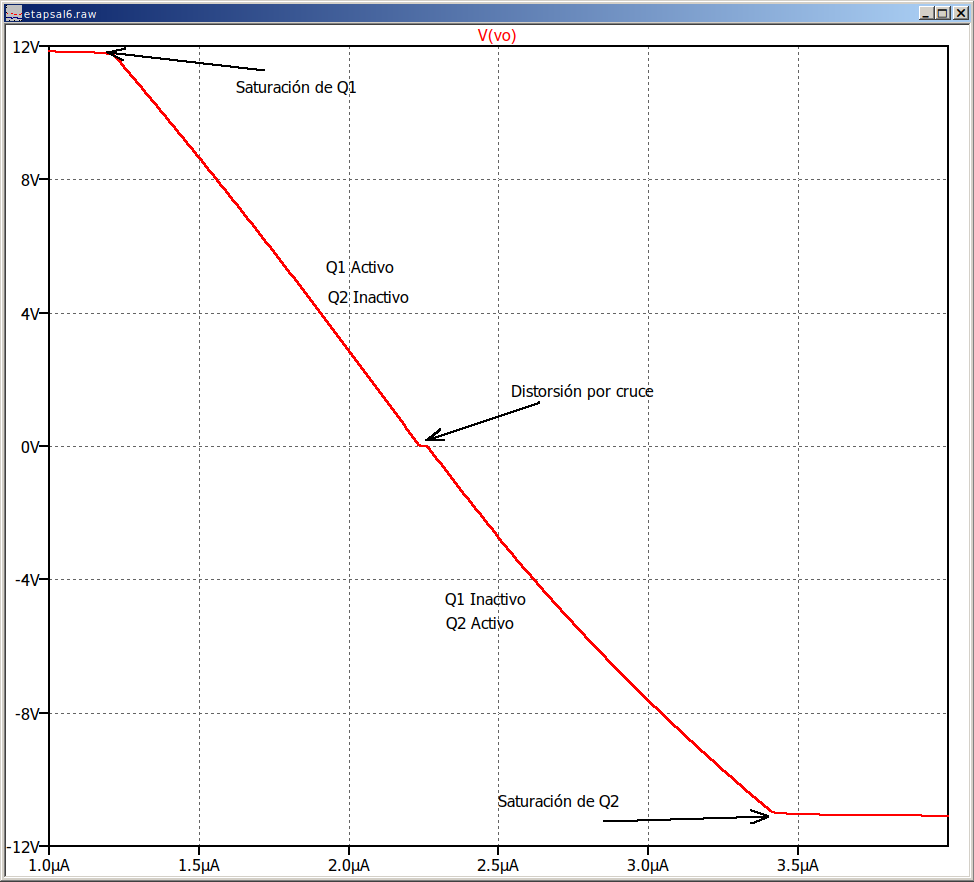
\includegraphics[width=0.8\linewidth]{figuras/claseabyc9.png}
	\caption{Respuesta temporal de una etapa clase B controlada por corriente.}
	\label{clases9}
\end{figure}



En circuitos prácticos, la distorsión por cruce es en general un inconveniente que debe ser solucionado. En las configuraciones Clase B mostradas los transistores están polarizados con una tensión base emisor igual a cero, necesitando una tensión $V_{BE} = V_{BE}(on)$ para comenzar a conducir. Para mejorar esta situación se les suele dar a los transistores de salida una polarización al borde de la conducción, es decir $V_{BE} \approx V_{BE}(on)$, conduciendo éstos algo más de medio ciclo. Esta variante en la configuración de salida es la que
se denomina Clase AB. 

En la figura \ref{clases10} se muestran dos ejemplos posibles de implementaciones de etapas de salida Clase AB. En el circuito de la izquierda de la figura los transistores de salida están polarizados con sus respectivas tensiones base emisor producidas por la caída en la resistencia $R_1$ de $\approx 2V_{BE}(on)$. En el circuito de la izquierda se logra el mismo objetivo mediante las caídas en los dos diodos $D_1$ y $D_2$, esta última implementación tiene la ventaja de lograr una compensación con respecto a las variaciones de temperatura, ya que al variar ésta, varían las tensiones base emisor de los transistores y en los diodos en forma similar, produciéndose una compensación.

En la figura \ref{clases11} se muestra la transferencia de la etapa de salida Clase AB del circuito implementado con diodos, en la que se muestra como se mejora notablemente la distorsión por cruce. En el caso del circuito implementado a la izquierda se producen resultados similares.

 \begin{figure}
	\centering
	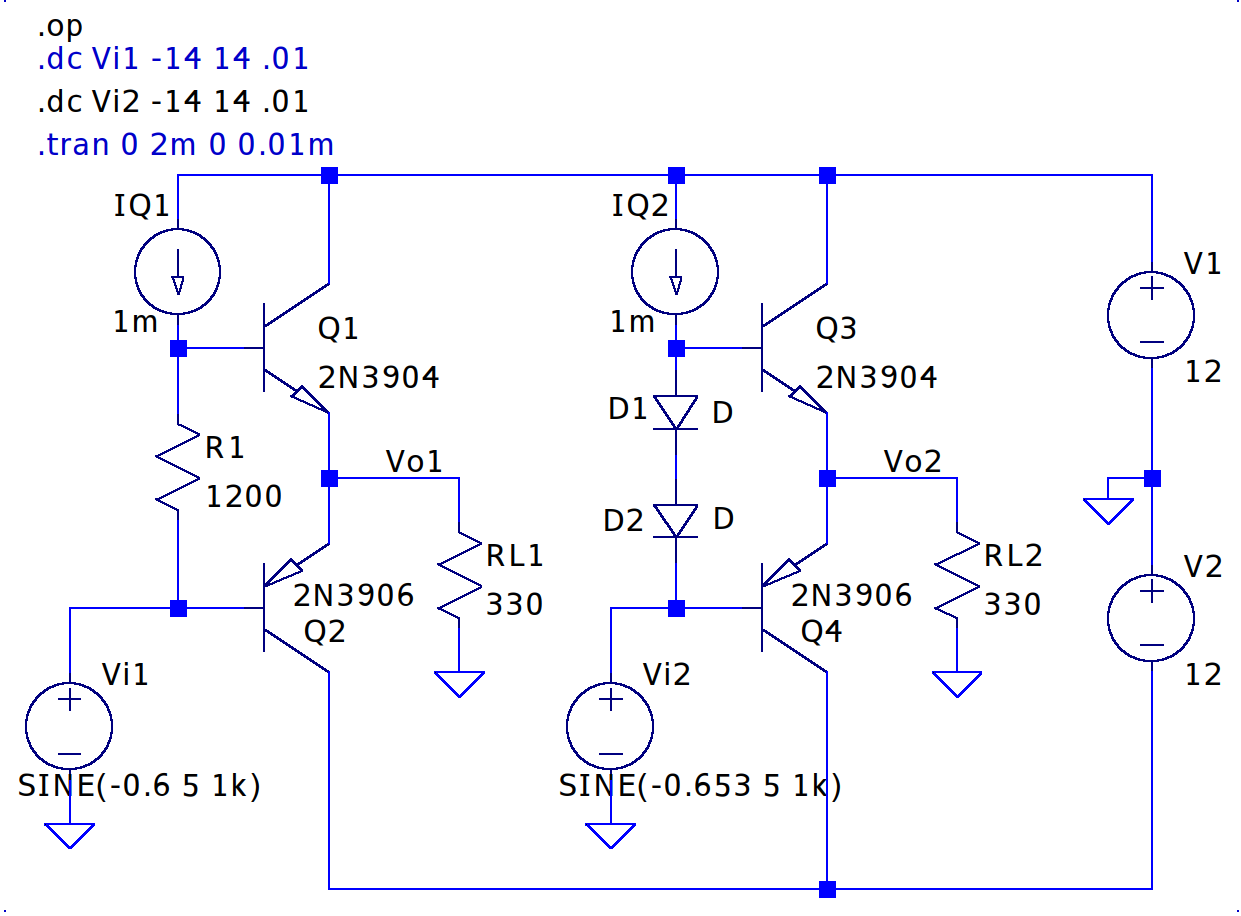
\includegraphics[width=0.8\linewidth]{figuras/claseabyc10.png}
	\caption{Configuraciones de salida Clase AB. Mejora de la distorsión por cruce}
	\label{clases10}
\end{figure}

 \begin{figure}
	\centering
	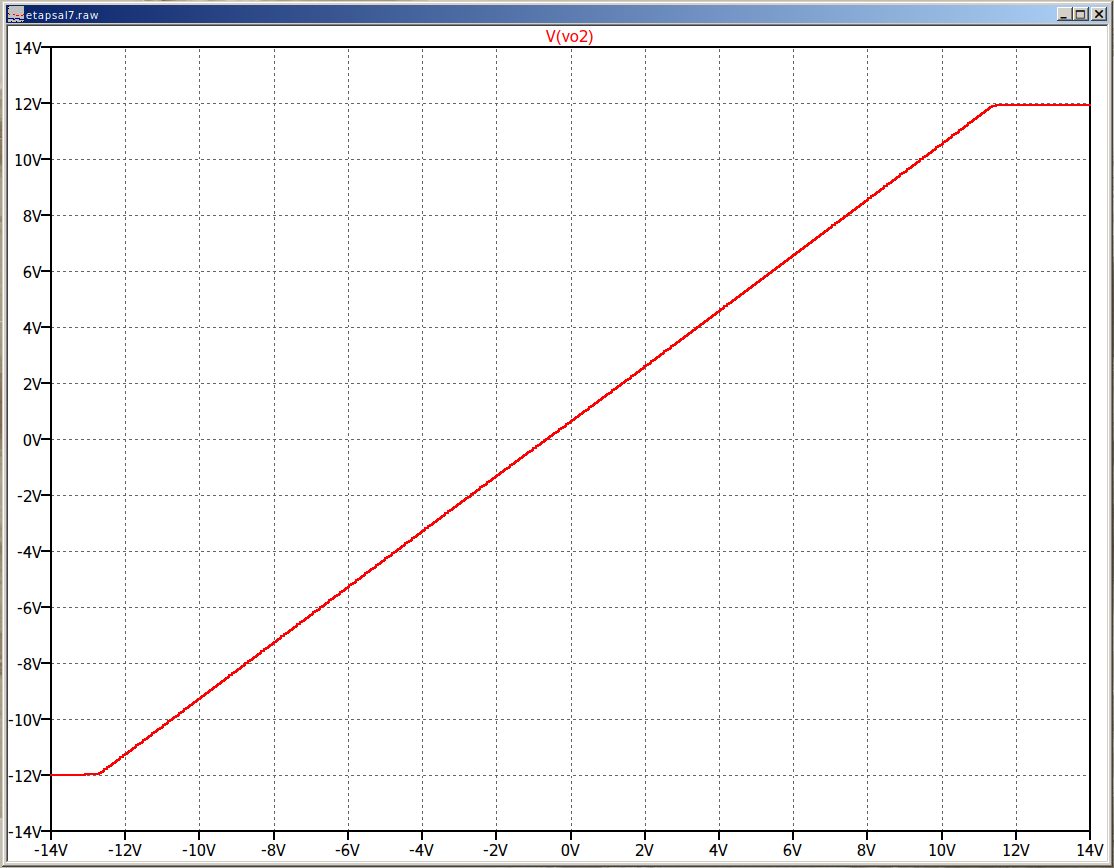
\includegraphics[width=0.8\linewidth]{figuras/claseabyc11.png}
	\caption{Transferencia de una etapa clase AB con diodos. }
	\label{clases11}
\end{figure}

El circuito de la figura \ref{clases12} es un ejemplo de un amplificador de potencia Clase AB con etapa preamplificadora implementada con un amplificador operacional y realimentación negativa dada por las resistencias $R_2$ y $R_3$. La ganancia de tensión a frecuencias medias es $|\displaystyle \frac{V_o}{V_i}| \approx 1+\displaystyle \frac{R_2}{R_3}$ y la potencia de salida es manejada por $Q_1$ y $Q_2$. La figura \ref{clases13} es la respuesta temporal a una tensión senoidal de entrada de frecuencia $1KHz$  y de amplitudes de $0,5V$ y $1V$ respectivamente. En la curva roja se ve la respuesta lineal con la ganancia adecuada (para $\hat{V}_i=0,5V$) y en la azul se ven los límites de la máxima excursión simétrica producidos por la saturación de los dispositivos ($\hat{V}_i=1V$).
En forma similar a como se obtuvieron las potencias medias puestas en juego en la etapa de salida Clase A, se pueden obtener las mismas en este circuitos dando valores similares a los que se pueden calcular teóricamente.

 \begin{figure}
	\centering
	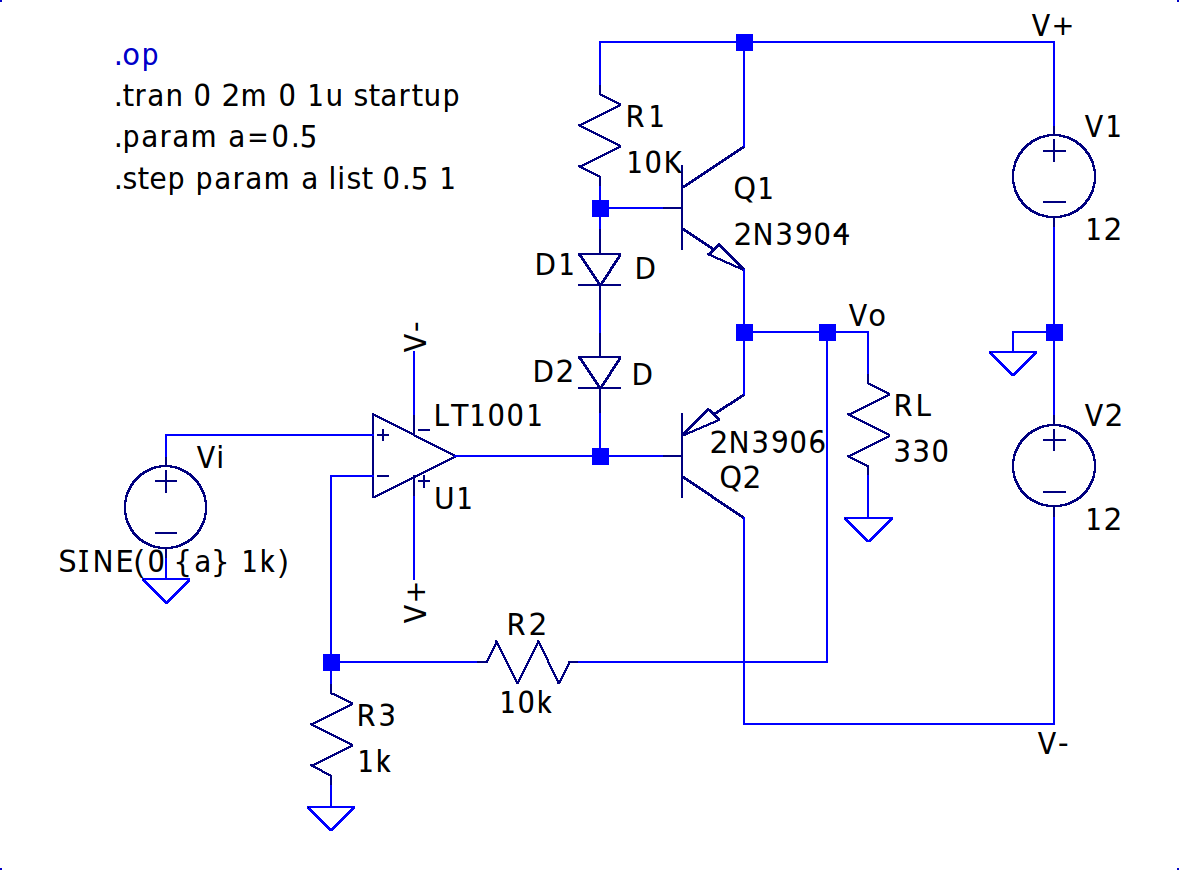
\includegraphics[width=0.8\linewidth]{figuras/claseabyc12.png}
	\caption{Ejemplo de Amplificador de Potencia Clase AB}
	\label{clases12}
\end{figure}

\begin{figure}
	\centering
	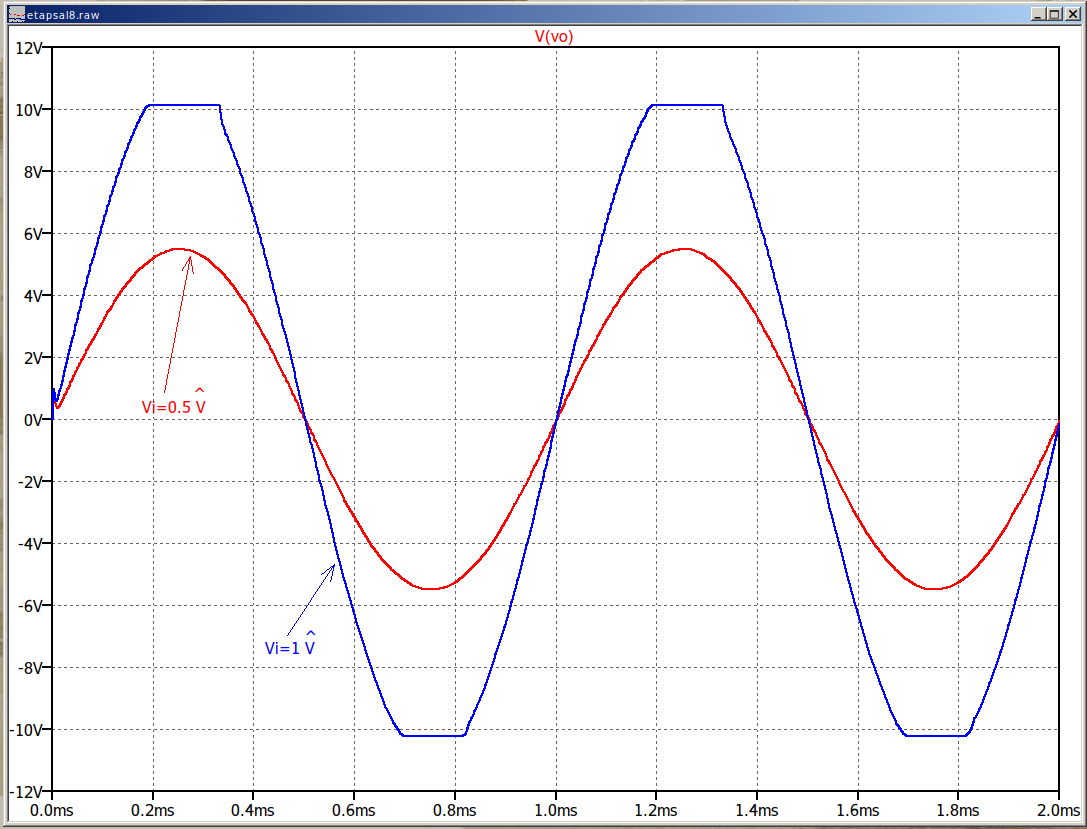
\includegraphics[width=0.8\linewidth]{figuras/claseabyc13.png}
	\caption{Respuestas temporales del ampliificador Clase AB. }
	\label{clases13}
\end{figure}


